\chapter{Interférométrie}

\section{L'interféromètre de Fabry-Perot}
L’interféromètre de Fabry-Peret est composé de deux petits miroirs placés parallèlement l'un à 
l'autre et à distance contrôlée. Étudions ce dispositif à travers la lumière passant à travers 
deux miroirs\footnote{En réalité, la lumière passant à travers, il s'agit de \textit{semi-miroirs}.} 
parallèles.\\

	\begin{wrapfigure}[6]{l}{5cm}
	\vspace{-5mm}
	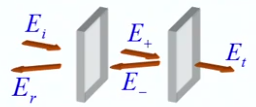
\includegraphics[scale=0.5]{ch4/image1.png}
	\captionof{figure}{ }
	\end{wrapfigure}
Le champ incident $E_i$ est partiellement transmis ($E_+$) et réfléchi ($E_r$). Il arrive sur 
le deuxième miroir où une partie est réfléchie dans la \textit{cavité optique} $E_-$ et une transmise 
par delà le second miroir, $E_t$. Le champ réfléchi $E_r$ comprend la contribution de l'ensemble 
du système comme nous le verrons plus tard. \\

	\begin{wrapfigure}[8]{r}{4.2cm}
	\vspace{-5mm}
	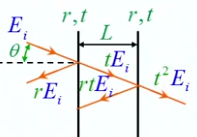
\includegraphics[scale=0.65]{ch4/image2.png}
	\captionof{figure}{ }
	\end{wrapfigure}
On peut s'intéresser aux \textit{réflexions multiples}. Représentons des miroirs comme 
des lames infiniment minces décrites par des coefficients de réflexion et transmission $r$ et $t$. 
On s'intéresse au cas du Fabry-Perot symétrique : les deux miroirs sont identiques, placés à une 
distance $L$. Un champ $E_i$ arrive sur le premier miroir à un angle d’incidence $\theta$ par 
rapport à la normale\footnote{Ce champ n'est pas "ponctuel" comme un laser mais bien une onde 
plane, comme le montre le schéma ci-dessus.}. Le coefficient de réflexion en amplitude $r$ nous 
donne le champ réfléchi : $rE_i$. De même, pour la transmission, $tE_i$ ect. pour le second miroir.\\

	\begin{wrapfigure}[8]{l}{4.2cm}
	\vspace{-5mm}
	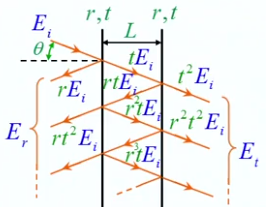
\includegraphics[scale=0.45]{ch4/image3.png}
	\captionof{figure}{ }
	\end{wrapfigure}
En suivant un raisonnement analogue pour le faisceau "dans" la cavité optique, il faut tenir compte 
les réflexions multiples qui contribuent aux champs totaux réfléchi $E_r$ et transmis $E_i$. On obtient 
alors une suite infinie de champs à considérer : principe de superposition. On pourrait étudier la 
convergence de la série mais nous allons quitter l'approche des réflexions multiples au profit d'une 
\textit{approche globale}.\\

	\begin{wrapfigure}[8]{r}{3cm}
	\vspace{-5mm}
	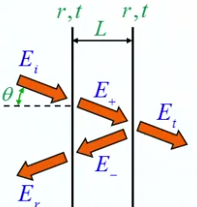
\includegraphics[scale=0.45]{ch4/image4.png}
	\captionof{figure}{ }
	\end{wrapfigure}
Considérons également un champ $E_i$ arrivant à un angle $\theta$. Par contre, dans la cavité, on 
considère un champ $E_+$ désignant l'ensemble des champs qui se propage dans le même sens que 
$E_i$ (dans $E_i$ se cache la somme $(t+rt+r^2t+\dots)E_i$). Ce $E_+$ engendre un champ $E_-$, soit 
la somme de toutes les ondes planes se déplaçant vers la gauche. Forcément, il y aura la 
transmission du champ $E_+$ donnant le champ transmis du Fabry-Perrot, $E_t$.\\

Pour connaître $E_t$, il faut passer par le calcul de $E_+$ et déduire le champ transmis par la 
transmission de $E_+$ : $E_t=tE_+$. De même, pour la réflexion : $E_r = rE_i+tE_-$. On ne fait 
rien d'autre que d'appliquer le principe de superposition.\\

	\begin{wrapfigure}[10]{l}{3.5cm}
	\vspace{-5mm}
	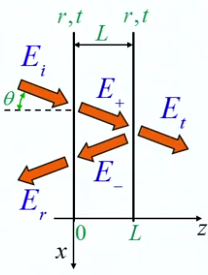
\includegraphics[scale=0.45]{ch4/image5.png}
	\captionof{figure}{ }
	\end{wrapfigure}
Faisons maintenant les choses de façon précises : on cherche à exprimer le champ transmis du 
Fabry-Perrot en fonction du champ incident. Bref, on cherche le "fonction de transfert". Pour 
commencer, il nous faut l'expression des champs eux-mêmes. Ce sont des ondes planes
\begin{equation}
\left\{\begin{array}{ll}
E_+ = \DS A_+e^{i\beta z}e^{i\rho x}\\
E_- = \DS A_-e^{-i\beta z}e^{i\rho x}
\end{array}\right.
\end{equation}
L'axe $x$ a été dirigé vers le bas afin que $\rho$, la projection du vecteur d'onde sur l'axe 
des $x$ soit positive, ayant choisi un rayon qui descend. Le $\beta$ représente ainsi la 
projection du vecteur d'onde sur l'axe $z$
\begin{equation}
\beta = k\cos\theta,\qquad \rho = k\sin\theta
\end{equation}
Pour l'onde réfléchie, on retrouve $-i\beta z$, l'onde se propageant vers les $z$ négatifs. 
Introduisons les conditions aux limites de cavité en tenant compte de l'endroit où cette 
condition est exprimée

\retenir{\ \textbf{Conditions aux limits de "cavité"}
\begin{enumerate}
\item $$E_t = tE_+(L) = tE_+(0)e^{i\beta L}$$
En effet, le champ en $L$ peut être exprimé avec celui en 0 (cf. système d'équation ci-dessus).
Les $e^{i\rho x}$ se simplifient : il ne faut pas en tenir compte (invariance sur l'axe $x$), 
nous ne tiendrons compte que des phases. 
\item $$E_+(0) = tE_i+rE_-(0)$$
Il ne faut pas oublier la réflexion de $E_-$ en 0 qui vient "nourir" $E_+$.
\item $$E_-(0) = rE_+(L)e^{i\beta L} = rE_+(0)e^{2i\beta L}$$
Il s'agit de la réflexion de $E_+$ en $L$ mais en rajoutant toute la phase de propagation. 
S'il n'y a pas de signe négatif dans l'exponentielle, c'est parce que nous allons de $L$ en 
zéro.
\end{enumerate}}\ \\

Si l'on ne s'intéresse pas à $E_r$, nous avons trois inconnues : ces CL sont suffisantes. 
Considérons les combili de ces CL. En combinant (2) et (3)
\begin{equation}
E_+(0) = tE_i+r^2e^{2i\beta L}E_+(0)\quad\Leftrightarrow\quad E_+(0)[1-r^2e^{2i\beta L}] = tE_i
\end{equation}
L'inconnue étant éliminée, on trouve
\begin{equation}
E_+(0) = \dfrac{tE_i}{\DS 1-r^2e^{\DS 2i\beta L}}
\end{equation}
Il reste la CL (1) pour la transmission. En multipliant de part et d'autre par $te^{i\beta L}$
\begin{equation}
E_t = \dfrac{t^2E_i\ e^{i\beta L}}{\DS 1-r^2e^{2i\beta L}} = T_{FP}\times E_i
\end{equation}
On peut alors définir la fonction de transfert du Fabry-Perot. Tout le comportement du FP est 
exprimé dans cette fonction (pour la transmission).
\begin{equation}
T_{FP} = \dfrac{t^2\ e^{i\beta L}}{\DS 1-r^2e^{2i\beta L}}
\end{equation}
Intéressons-nous aux intensités
\begin{equation}
E_t = T_{FP}\times E_i\quad\Rightarrow\quad |E_t|^2 = |T_{FP}|^2 \times |E_i|^2
\end{equation}
où $|T_{FP}|^2 = \mathcal{T}$, la fonction de transmission en intensité.\\

Faisons une petite parenthèse : introduisons la fonction de transmission en intensité pour 
un miroire simple. Dans ce cas $E_t = tE_i$. Dès lors
\begin{equation}
|E_t|^2 = t^2|E_i|^2
\end{equation}
La \textit{transmission en intensité du miroir} vaut $T=t^2$. De même pour la \textit{réflectivité} 
$R=r^2$. Ceci permet d'introduire des concepts nouveaux. Partons de la conservation de l’énergie 
(supposé sans pertes, miroirs parfaits)
\begin{equation}
|E_t|^2+|E_r|^2=|E_i|^2
\end{equation}
Ceci donne lieu à une relation particulière entre $T$ et $R$
\begin{equation}
T|E_i|^2+R|E_i|^2 = |E_i|^2\qquad\Longrightarrow\qquad T+R=1
\end{equation}
C'est la conservation de l'énergie pour un miroir parfait. On peut ré-écrire la fonction de 
transmission compte-tenu de ceci :
\begin{equation}
T_{FP} = \dfrac{(1-R)e^{i\beta L}}{1-Re^{2i\beta L}}
\end{equation}
Fin de la parenthèse, revenons à nos moutons : exprimons $\mathcal{F}$ 
\begin{equation}
\mathcal{F} = \dfrac{(1-R)^2}{|1-R[\cos(2\beta L)+i\sin(2\beta L)]|^2}
\end{equation}
En calculant le dénominateur
\begin{equation}
\mathcal{F} = \dfrac{(1-R)^2}{[1-R\cos(2\beta L)]^2+R^2\sin^2(2\beta L)} = \dfrac{(1-R)^2}{
1-2R\cos(2\beta L)+R^2\cos^2(2\beta L)+R^2\sin^2(2\beta L)}
\end{equation}
Avec l'identité fondamentale
\begin{equation}
\mathcal{T} = \dfrac{(1-R)^2}{1-2R\cos(2\beta L)+R^2}
\end{equation}
Sachant que $\cos(2\theta) = 1-2\sin^2(\theta)$
\begin{equation}
\mathcal{T} = \dfrac{(1-R)^2}{\underbrace{1-2R+R^2}_{(1-R)^2}+4R\sin^2(\beta L)} = 
\dfrac{1}{1+\dfrac{4R\sin^2(\beta L)}{(1-R)^2}}
\end{equation}
En posant $\DS F=\frac{4R}{(1-R)^2}$, la \textit{finesse} du FB.


\retenir{\ \textbf{Fonction d'Airy}
\begin{equation}
\mathcal{T} = \dfrac{1}{1+F\sin^2(\beta L)}
\end{equation}
Ceci caractérise le FB en fonction de l'intensité lumineuse.}\ \\

Rappelons 
\begin{equation}
F = \dfrac{4R}{(1-R)^2},\qquad \beta = k_0\cos\theta
\end{equation}
Choisissons $R=0.17$ tel que $F = 1$. Nous pouvons alors représenter $\mathcal{T}$ 
graphiquement. Il s'agit d'une fonction périodique de fonction $\pi$, le sinus étant 
au carré. Aux multiples de $\pi$, on récupère une transmission unitaire. Entre les pics, on 
obtient un minimum pour $(2n+1)\frac{\pi}{2}$.  

\begin{center}
	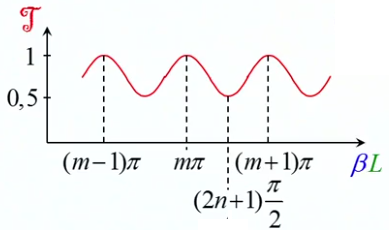
\includegraphics[scale=0.45]{ch4/image6.png}
	\captionof{figure}{ }
\end{center}

On peut maintenant s'intéresser à la réflexion. En définissant la fonction de transmission 
en intensité du FB 
\begin{equation}
|E_r|^2 = \mathcal{R}\times|E_i|^2
\end{equation}
Pas besoin de chercher de 12 à 14h : $\mathcal{R}+\mathcal{T}=1$, les miroirs étant sans 
pertes. 

\begin{center}
	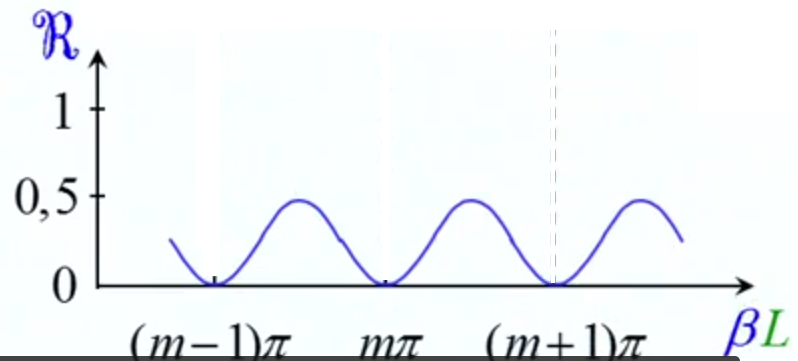
\includegraphics[scale=0.25]{ch4/image7.png}
	\captionof{figure}{ }
\end{center}

Ceci montre que lorsque $\beta L = n\pi$, nous aurons un zéro. Ce résultat est totalement 
indépendant de $R$ et $F$. Dès lors, en prenant un miroir où $R=99.99\%$ de réflexion, 
toute la lumière qui arrive passe au travers. C'est une belle surprise. 

\newpage
\section{L'interféromètre de Fabry-Perot : interprétation physique}
Le but est d'interpréter ce qui se passe physiquement lorsque $\beta L$ est un multiple de 
$\pi$, ou tout est transmis malgré un coefficient de réflexion proche de l'unité. Pour se 
faire, partons de la formule de $T_{FP}$ écrite dans le cas où $\beta L = m\pi$.
\begin{equation}
T_{FP} = \frac{t^2(-1)^m}{1-r^2} = (-1)^m
\end{equation}

	\begin{wrapfigure}[10]{l}{6.5cm}
	\vspace{-5mm}
	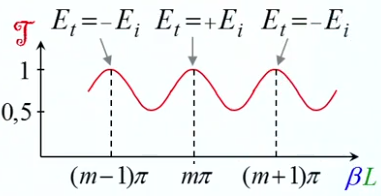
\includegraphics[scale=0.45]{ch4/image8.png}
	\captionof{figure}{ }
	\end{wrapfigure}
où l'on a utilisé $t^2 = 1-r^2$ (miroirs idéaux). Ceci nous montre quelque chose d'un peu 
plus subtil au niveau du champ transmis (alternance de phase). Si $m$ est pair, le champ 
transmi vaut le champ incident et pour les valeurs impaires l'opposé (déphasage de 180 degré 
entre la champ incident et transmis). Il y a des effets de phases en passant d'un pic à l'autre 
de la fonction de Airy. \\

Intéressons-nous maintenant au champ réfléchi : comment pouvons nous avoir aucune réflexion 
sur un miroir possédant un coefficient de réflexion proche de l'unité ?
\begin{equation}
E_r = rE_i+tE_-(0)
\end{equation}
Ce champ est composé de la partie directement réfléchie du champ incident ainsi que de la 
transmission du champ $E_-$ en zéro (\danger). Rappelons-nous la troisième condition aux 
limites de "cavité : $E_-(0) = rE_+(L)e^{i\beta L} = rE_+(0)e^{2i\beta L}$. Celle-ci donne 
l'expression de $E_-$ en fonction de $E_+(0)$. Or, la première condition ($E_t = tE_+(L) = 
tE_+(0)e^{i\beta L}$) peut exprimer $E_+$ en fonction de $E_t$ qui, lui, est connu.\\

Allons-y
\begin{equation}
\begin{array}{lll}
E_r &= rE_i+tE_-(0) &= rE_i +rtE_+(0)e^{2i\beta L}\\
&= rE_i + rE_te^{i\beta L} &= rE_i+rT_{FP}e^{i\beta L}E_i
\end{array}
\end{equation}
où, pour la dernière égalité, on a utilisé $E_t = T_{FP}E_i$. Nous avons bien exprimé le 
champ réfléchi en fonction du champ incident. En remplaçant $T_{FP}$ par son expression
\begin{equation}
E_r = rE_i + r\frac{t^2e^{2i\beta L}}{1-r^2e^{2i\beta L}}E_i
\end{equation}
Considérons cette expression à la résonance (cf. plus bas), soit en $\beta L = m\pi$. 
Les exponentielles valent 1 et les miroirs étant parfait, on obtient
\begin{equation}
??\quad E_r = 2rE_i\quad ??
\label{eq:ptint}
\end{equation}
Or,ce n'est pas ce que l'on obtient en regardant $\mathcal{R}$, nous devrions avoir zéro. 
Mathématiquement tout est correct, l'usage de celles-ci l'est moins (l'erreur se situe au 
niveau des simplification donnant lieu à \eqref{eq:ptint}). Nous avons fait une 
erreur sur l'interprétation physique des coefficients de réflexion et transmission. Un 
miroir est plus subtil que ça. Voyons le.

\newpage
	\begin{wrapfigure}[6]{l}{4cm}
%	\vspace{-5mm}
	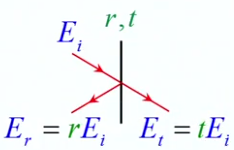
\includegraphics[scale=0.45]{ch4/image9.png}
	\captionof{figure}{ }
	\end{wrapfigure}
Reconsidérons le miroir vu précédemment : $E_r = rE_i$ et $E_t=tE_i$. Ces champs sont 
électromagnétiques, on peut écrire les équations de Maxwell. En faisant ça, on voit directement 
que l'équation d'onde est invariante par rapport à un renversement du temps : $t^2$ est 
"insensible" au changement $t'=-t$.
\begin{equation}
\Delta E = \mu_0\epsilon_0\dfrac{\partial^2E}{\partial t^2} = \mu_0\epsilon_0\dfrac{\partial^2 E}{
\partial (-t)^2}
\end{equation}

	\begin{wrapfigure}[7]{r}{3.5cm}
	\vspace{-5mm}
	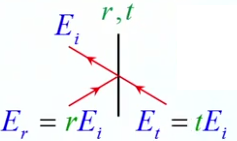
\includegraphics[scale=0.45]{ch4/image10.png}
	\captionof{figure}{ }
	\end{wrapfigure}
Les raisonnements fait pour les faisceaux allant dans un sens sont valable dans l'autre. Le 
raisonnement tenu plus haut doit être valable si on "inverse" le temps (ce qui revient ici à 
inverser le sens de propagation des faisceaux). La situation ci-contre doit être identique à 
celle obtenue ci dessus, à gauche. Le faisceau transmis joue le roule du faisceau incident. Or, 
le champ réfléchi joue le roule d'un second faisceau incident, c'est la recombinaison des 
deux qui doit donner $E_i$. Or, si on réalise cette expérience, $E_t$ va donner un champ transmis
qui vaudra $t^2 E_i$, pour le champ réfléchi on obtiendra $r^2 E_i$. Si les équations de 
Maxwell sont vraiment invariante pour un inversement du temps, on devrait avoir
\begin{equation}
t^2E_i+r^2E_i = E_i
\end{equation}

	\begin{wrapfigure}[6]{l}{3cm}
	\vspace{-15mm}
	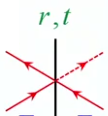
\includegraphics[scale=0.65]{ch4/image11.png}
	\captionof{figure}{ }
	\end{wrapfigure}
Comme $t^2+r^2=1$, l'égalité est vérifiée. Mais en faisant cette expérience, il y aura une 
partie transmise et réfléchie : celles-ci sont-elles nulles (en pointillé, ci-contre) ? Ce 
champ en pointillé est donné par
\begin{equation}
rtE_i + trE_i = 2tr E_i \neq 0
\end{equation}
Il y a à priori un souci et ce parce que nous avons négligé quelque d'important : lorsque l'on 
considère la réflexion d'un côté d'un miroir on a un certain coefficient de réflexion $r$, 
automatiquement, lorsqu'on a la réflexion de l'autre coté du miroir on a un coefficient qui 
vaut $-r$. On observe alors bien zéro. Si on nomme un coefficient $r$ d'un côté, il faut le 
nommer $-r$ de l'autre : il y a toujours un déphasage de 180$^\circ$ du champ d'un côté par 
rapport à l'autre du miroir. \\

Il faut en tenir compte. Or pour le moment, on a toujours considéré des coefficients de 
réflexion positif et ce même à l'intérieur de la cavité. La réflexin à l'intérieur doit 
être décrite par $"-r"$ de sorte à obtenir
\begin{equation}
\begin{array}{lll}
E_r &= -rE_i+tE_-(0) &= -rE_i +rtE_+(0)e^{2i\beta L}\\
&= rE_te^{i\beta L} &= -rE_i+rT_{FP}e^{i\beta L}E_i
\end{array}
\end{equation}
En refaisant les mêmes simplifications, on obtient cette fois-ci 
\begin{equation}
E_r = 0
\end{equation}
Ceci est le résultat d'interférences destructives entre ce qui est directement réfléchi
du faisceau incident et ce qui est transmis du champ $E_-$. C'est ça qui crée cette 
possibilité d'avoir un champ nul même avec $r=0.99$. Nous avons bien une interférence 
destructives entre ces deux champ et si rien n'est réfléchi, c'est que tout est transmis.\\

Continuons l'analyse de la fonction de transmission en analysant ce qui se passe autour de 
$\beta L = m\pi$. Par définition $\beta = k\cos\theta$
\begin{equation}
\beta = k\cos\theta\quad\Rightarrow\quad kL\cos\theta = m\pi\quad\Leftrightarrow\quad 
\dfrac{2\pi}{\lambda}L\cos\theta = m\pi
\end{equation}
Ceci nous donne une condition entre $L$ et $\lambda$. Après simplifications
\begin{equation}
L = \frac{m}{2}\frac{\lambda}{\cos\theta}
\end{equation}

	\begin{wrapfigure}[7]{r}{4.5cm}
	\vspace{-5mm}
	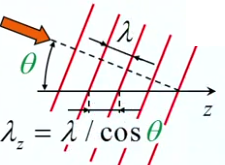
\includegraphics[scale=0.55]{ch4/image12.png}
	\captionof{figure}{ }
	\end{wrapfigure}
La longueur est dans un certain rapport avec la longueur d'onde faisant intervenir un 
angle $\theta$. Le rapport $\lambda/\cos\theta$ est intéressant physiquement. Nous avons 
des ondes planes qui se propage avec un certain angle $\theta$ par rapport à l'axe $z$. Ce 
rapport est tout simplement la longueur d'onde de la lumière le long de l'axe $z$. L’écart 
entre deux front d'onde ($\lambda$ dans la direction de l'onde) vaudra quelque chose de plus 
grand que $\lambda$, soit $\lambda_z = \lambda/\cos\theta$ lorsqu'il est projeté sur l'axe $z$.\\

On a une périodicité en $z$ qui est imposée par $\beta$ et non pas par $k$. Reprenons :
\begin{equation}
\beta L = kL\cos\theta = m\pi
\end{equation}
La condition porte sur $\beta L$, cela porte bien sur les \textbf{déphasages} de l'onde au 
travers de la cavité de longueur $L$. On aurait tendance à dire que le déphasage accumulé 
sur la longueur $L$ est d'autant plus grand que $\theta$ est important, la distance devenant 
de plus en plus grande. On aurait alors tendance, à tort, de se dire que la phase accumulée est 
d'autant plus grande que que la phase est grande. C'est le contraire : plus $\theta$ est grand, 
plus $\lambda_z$ devient grand et la phase accumulée devient petite. Nous avons bien $\cos\theta$ 
et non pas $1/\cos\theta$.\\

Une autre façon de voir les chose est de se dire que $\lambda_z$ est la périodicité de l'onde 
évoluant en $e^{i\beta z}$
\begin{equation}
\frac{2\pi}{\beta} = \lambda_z = \lambda\cos\theta
\end{equation}
L'erreur est donc de considérer l'accumulation sur le chemin optique et non pas sur la longueur 
de la cavité.\\

Fermons la parenthèse et écrivons plutôt
\begin{equation}
L = m\frac{\lambda_z}{2}
\end{equation}
C'est une façon de traduire la condition de résonance$\beta L = m\pi$ : la longueur de la cavité 
doit être un multiple de la demi-longueur d'onde. Il s'agit de la condition de formation d'une onde 
stationnaire. Une corde fixée aux extrémités peut vibrer selon différents modes, défini en fonction 
du point ou on excite mécaniquement la corde. Quand $\beta L = m\pi$, on forme des ondes stationnaires.\\

	\begin{wrapfigure}[9]{l}{5cm}
	\vspace{-5mm}
	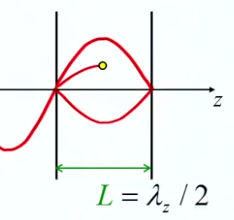
\includegraphics[scale=0.60]{ch4/image15.png}
	\captionof{figure}{ }
	\end{wrapfigure}
Représentons l'onde incidence (branche du cosinus, $e^{i\beta z}$ au temps $t=z=0$ soit 1, la C.I.). En 
passant à travers du miroir, cette onde se voit atténuée mais le front d'onde continue de se propager. 
On atteint ensuite le second miroir où l'onde réfléchie va également être atténuée. Une fois arrivé au 
second miroir, on commence à voir les interférences constructives : on forme une onde stationnaire avec 
un nœud au centre et deux demi-ventres. Une fois revenue au premier miroir, elle va être réfléchie et 
atténuée. Mais cette nouvelle onde réfléchie sera en phase avec l'onde réfléchie au second miroir. 
En continuant, on aura par interférences constructives, la formation d'un champ important.\\

Étudions maintenant ce qui se passe au niveau du champ de cavité. Pour obtenir l'amplitude de l'onde 
intracavité $E_+$ (la somme de toutes les ondes qui vont dans le même sens, ici vers la droite), partons de 
\begin{equation}
E_t = t E_+(L)\quad\Rightarrow\quad|E_t|^2 = T|E_+|^2
\end{equation}
Travaillons en intensité. C'est facile car $E_t=E_i$ à la résonance car $\mathcal{T}=1$.
\begin{equation}
|E_i|^2 = T|E_+|^2
\end{equation}
L'intensité de cavité est donnée par 
\begin{equation}
|E_+|^2 = \frac{|E_i|^2}{T}
\end{equation}

	\begin{wrapfigure}[11]{l}{6.5cm}
	\vspace{-15mm}
	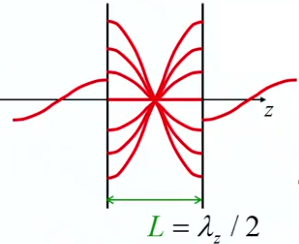
\includegraphics[scale=0.60]{ch4/image13.png}
	\captionof{figure}{ }
	\end{wrapfigure}
Or, $T$ peut être très petit. Si $T=0.001$, l'intensité dans la cavité peut être 1000 fois plus 
importante que celle du champ incident. On aura toujours un champ renforcé dans la cavité
\begin{equation}
|E_+|^2> |E_i|^2
\end{equation}
Dans un FB, on observe un phénomène résonance comparable à celui obtenu pour la vibration d'une 
corde : un petite amplitude d'excitation mécanique peut donner lieu à une grande oscillation de 
la corde. A la sortie du FB on a bien une petite amplitude, la transmission atténue fortement le 
champ.\\


	\begin{wrapfigure}[11]{r}{6cm}
	\vspace{-5mm}
	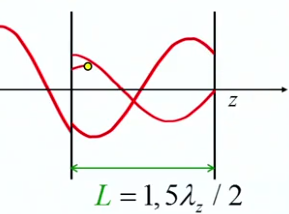
\includegraphics[scale=0.60]{ch4/image14.png}
	\captionof{figure}{ }
	\end{wrapfigure}
Pour se convaincre de l'interprétation physique, regardons le cas ou $\beta L = (2m+1)\frac{\pi}{
2}$, c'est-à-dire la ou nous avions les maxima de la fonction de réflexion. En suivant un raisonement 
similaire
\begin{equation}
L = \frac{(2m+1)\lambda_z}{4}
\end{equation}
Dans ce cas la, l'onde réfléchie par le premier miroir est en opposition de phase par rapport à l'onde 
transmise de l'onde incidente. Il s'agit d'une \textit{anti-résonance} : très peu sera transmis et le 
maximum sera réfléchi\footnote{Pq ?}.



\newpage
\section{Optique des films minces}
On va se contenter d'expliquer l'origine de la décomposition en couleur de la lumière blanche, 
par exemple sur une bulle de savon. Un film mince représente un FP d'épaisseur $L$ (on regarde 
la bulle de très près de façon à l'avoir rectiligne).

\begin{center}
\vspace{-5mm}
	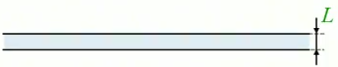
\includegraphics[scale=0.60]{ch4/image18.png}
	\captionof{figure}{ }
\end{center}

Le coefficient de réflexion est donnée par celui de Fresnel (l'indice de réfraction dans et 
en dehors de la bulle étant différent)
\begin{equation}
r = \frac{n_1-n_2}{n_1+n_2}
\end{equation}
	\begin{wrapfigure}[11]{l}{6cm}
	\vspace{-13mm}
	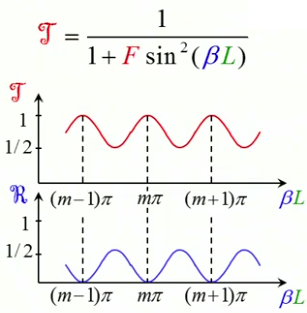
\includegraphics[scale=0.5]{ch4/image17.png}
	\captionof{figure}{ }
	\end{wrapfigure}
Cette réflexion est double, on a bien affaire à un FP. On peut le décrire avec sa fonction de 
Airy
\begin{equation}
\mathcal{F} = \dfrac{1}{F+\sin^2(\beta L)}
\end{equation}
Ceci est une forme un peu simplifiée, dans le cas ou les indices de réfractions valaient tous 
les deux l'unité. Que l'on considère cet indice ou pas, la physique sera la même (onde stationnaire, 
résonance,\dots). On va considérer que l'indice entre les deux surface est l'indice de l'air afin 
de garder les mêmes notations que celles utilisées pour le FP.\\

Nous allons surtout ici nous intéresser à la fonction de réflexion $\mathcal{R}$, le phénomène d'irisation 
ayant lieu à la réflexion. Analysons ce qui se produit à une résonance ($\mathcal{T}=1,\mathcal{R}=0$) 
\begin{equation}
\beta L = kL\cos\theta = \frac{2\pi}{\lambda} L\cos\theta = m\pi
\end{equation}
où $\theta$ est l'angle par rapport à la verticale (le futur angle d'incidence).\\

	\begin{wrapfigure}[11]{r}{6cm}
	\vspace{-5mm}
	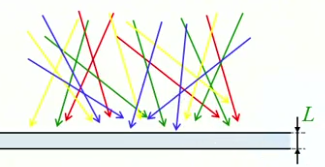
\includegraphics[scale=0.60]{ch4/image16.png}
	\captionof{figure}{ }
	\end{wrapfigure}
La longueur d'onde  
effective est bien donnée par $\lambda/\cos\theta$, la résonance correspond à une longueur valant 
un nombre entier de demi-longueur d'onde effective. Ce qui est intéressant est que $\lambda$ et 
$\theta$ apparaissent. La lumière venant de toutes les directions, tous les $\theta$ sont représentés.
On a également un certain nombre de longueur d'onde, toutes les longueurs d'ondes visibles sont à 
priori présentes. On est face à une situation un peu chaotique. Pourquoi irisation? Pourquoi certaines 
sont réfléchies plus que d'autres ? \\

	\begin{wrapfigure}[5]{l}{6cm}
	\vspace{-10mm}
	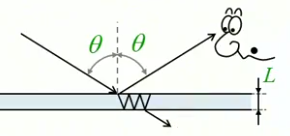
\includegraphics[scale=0.60]{ch4/image19.png}
	\captionof{figure}{ }
	\end{wrapfigure}
L'expérience est ici une observation, on forme une image. On observe la surface et en l'observant, on 
regarde un endroit de la surface : cela sélectionne un angle : la rayon qui arrive à l'oeil est un 
rayon qui a le même angle d'incidence mais de l'autre côté de la verticale. On observe un point 
parce qu'un rayon émane de ce point pour former une image sur notre rétine : on sélectionne une 
composante angulaire précise, $\theta$ est fixé.\\

Si $\theta$ et $L$ sont donnés, certains longueurs d'ondes vont être transmises par le FP. Cette 
transmission va être donnée pour une longueur d'onde particulière (même plusieurs, paramètre $m$)
\begin{equation}
\lambda_t = \dfrac{2L\cos\theta}{m}
\end{equation}
Analysons ce résultat en considérant $L=1\ \mu\text{m}, \theta = 60^\circ \rightarrow \cos\theta = 
0.5$. Ceci donne 
\begin{equation}
\lambda_t = \dfrac{2\times1\times 0.5}{m}\quad\Longrightarrow\quad \lambda_t = \frac{1}{m}\quad [\mu 
m]
\end{equation}
	\begin{wrapfigure}[7]{r}{6cm}
	\vspace{-5mm}
	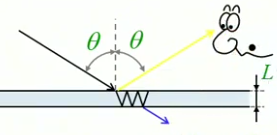
\includegraphics[scale=0.60]{ch4/image20.png}
	\captionof{figure}{ }
	\end{wrapfigure}
En considérant $m=1, \lambda_t=1\ \mu\text{m}$. Ceci se situe dans le domaine de l'infrarouge : 
celle-ci est totalement transmise et n'est pas visible (et de toute façon, elle ne l'était pas). 
Si $m=2, \lambda_t=0.5\ \mu$m, cela se situe dans le bleu. Pour $m=3$ on rentre dans l'ultraviolet. 
La longueur d'onde bleue est parfaitement transmise. L'observateur va donc observer de la lumière 
blanche sans le bleu, soit de la lumière jaune.\\

Le film mince à fait office de filtre, à la réflexion le bleu n'est plus présent. L'irisation n'est 
pas la vision de longueur d'onde pure comme c'est le cas pour l'arc-en-ciel. Nous allons percevoir 
une couleur jaune mais qui en réalité contient un grand nombre de longueur d'onde.\\

	\begin{wrapfigure}[8]{l}{6cm}
	\vspace{-5mm}
	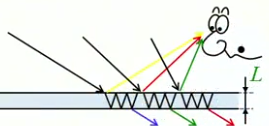
\includegraphics[scale=0.60]{ch4/image21.png}
	\captionof{figure}{ }
	\end{wrapfigure}
La rétine possède une certaine ouverture, les points d'à côtés seront également visibles. Considérons 
alors un angle $\theta = 55^\circ$. Pour $m=2$ on est dans le visible : $\lambda_t=0.57\mu$m (vert), 
soit une longueur d'onde plus grande. Le blanc moins le vert donne du rouge. En considérant un point 
encore un peu plus proche ($\theta =50^\circ$), on obtient $\lambda_t = 0.64\mu$m, soit du rouge qui 
donnera une couleur verte en réflexion. Allons plus loin, $\theta = 75^\circ\rightarrow \lambda_t = 0.5
\mu$m pour $m=1$, après ce n'est plus visible. \\

	\begin{wrapfigure}[15]{r}{4.5cm}
	\vspace{-5mm}
	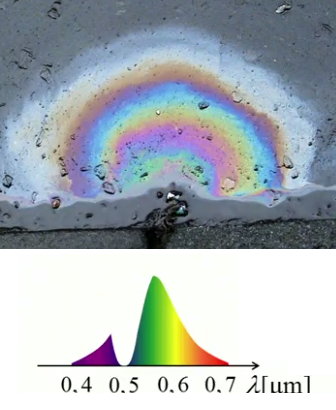
\includegraphics[scale=0.40]{ch4/image22.png}
	\captionof{figure}{ }
	\end{wrapfigure}
L'angle "déplace" la couleurs supprimée dans le spectre. Pour un angle lointain, il faut se limiter 
à l'ordre 1. Pour une distance moins loin, l'ordre 2 donne un longueur d'onde visible, \dots En 
pratique, c'est bien ce qui est observé. Chaque couleur représente des ordres différents (plus on 
ouvre en angle, plus l'ordre sera petit, si on recroise une couleur c'est son "ordre qui a été 
diminué".)\\

Mais que se passe-t-il pour un fil de l'ordre du centimètre, par exemple une plaque de verre. Nous 
avons donc $L=10^4\mu$m : le phénomène de sélection se produit toujours, mais il se fera sur des 
ordres de résonance très élevé ($m=10'000$). Pour le fun, étudions $m=2*10^4$. Pour un angle 
$\theta=60^\circ$ on obtient
\begin{equation}
\lambda_t = \frac{10^4}{m}
\end{equation}
Pour l'ordre $m$, on trouve $\lambda_t = 0.5\mu$m. L'ordre $m-1$ diffère très peu de cet ordre $m$ 
(différence au niveau de la cinquième décimale). Ceci signifie que les longueurs d'ondes passent 
à travers mais sont toutes très proches, ici dans le bleu. En répétant l'opération, il y a quelques 
20'000 réflexions qui ne sont plus réfléchie : le spectre est filtré avec une périodicité extrêmement 
serrée. Le résultat de ceci est qu'il y a un filtrage, mais l’œil n'est pas assez sensible : on 
verra toutes les couleurs du spectre visible et on ne verra pas le phénomène d'irisation ce qui est 
beaucoup moins drôle. Le phénomène de filtrage ne permet plus de couper des "grosses parties" du 
spectre visible. C'est pourquoi on ne voit pas d’irisation à sur les verres des lunettes.\\

	\begin{wrapfigure}[9]{r}{4.5cm}
	\vspace{-5mm}
	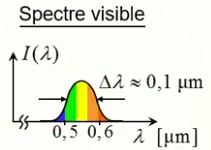
\includegraphics[scale=0.60]{ch4/image23.png}
	\captionof{figure}{ }
	\end{wrapfigure}
On peut expliquer ce phénomène d'une façon alternative en confrontant le spectre visible à la 
fonction de Airy. Ceci est assez naturel car la variable d'Airy, $\beta L$ renferme la longueur 
d'onde. Si le spectre visible à une certaine largueur ($\Delta \lambda \approx 0.1\mu$m) à 
$\theta, L$ fixé, une variation de longueur d'onde va donner une variation de la variable d'Airy 
$\beta L$. Prenons la différentielle
\begin{equation}
\beta L = \frac{2\pi}{\lambda} \cos\theta L\quad\Rightarrow\quad \frac{d}{d\lambda}(\beta L) =
-\frac{2\pi}{\lambda^2}\cos\theta L
\end{equation}
Ou encore, en exprimant la différentielle de la variable de Airy
\begin{equation}
d(\beta L) = -\frac{2\pi}{\lambda^2}d\lambda\cos\theta L
\end{equation}
Ceci donne une idée de l'extension du spectre visible $\Delta \lambda$ en terme de la variable 
de Airy $\beta L$. Exprimons maintenant cette relation pour des accroissements fini et non plus 
des différentielles.
\begin{equation}
\Delta(\beta L) = -\frac{2\pi}{\lambda^2}\Delta\lambda\cos\theta L
\end{equation}
Pour un angle et épaisseur donnée et pour la longueur d'onde visible (prenons $\lambda =0.5\mu$m, 
ce que l'on fait en général pour désigner la longueur d'onde "central" du visible). On trouve alors
\begin{equation}
\Delta (\beta L) =\frac{2\pi}{0.25}0.1\cos\theta L = 0.8\pi\cos\theta L
\end{equation}
Il s'agit de l’extension du spectre visible dans la variable d'Airy, nous allons pouvoir voir 
la place qu'occupe le spectre visible dans le graphique de la réflexion en fonction de $\beta L$.\\

	\begin{wrapfigure}[11]{l}{6.3cm}
	\vspace{-5mm}
	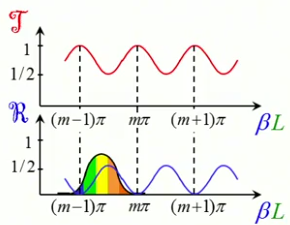
\includegraphics[scale=0.60]{ch4/image24.png}
	\captionof{figure}{ }
	\end{wrapfigure}
Considérons $L=1\mu$m $\rightarrow \Delta(\beta L) = 0.8\pi\cos\theta$. On obtient une grandeur 
qui vaut une fraction de fois $\pi$ : cette valeur est comparable à celle entre les résonance du FB, 
cet écart étant de $\pi$. Superposons les deux. Quelle est la position du spectre ? $\lambda$ et 
$L$ étant fixé, la position va uniquement dépendre de $\theta$.  On voit que la largeur doit dépendre 
de $\theta$, mais on ne rentre pas dans les détails. Lorsque l'angle $\theta$ (initialement important) 
diminue, on va "déplacer" son regard : le spectre visible se déplace vers la droite. En fonction de 
sa position, on peut voir ce qui est coupé et ce qui ne l'est pas.\\

\newpage
\textbf{Remarque} : pourquoi ce phénomène ne se fait-il que en réflexion? Si on n'en a pas, c'est 
parce que la profondeur de régulation (profondeur des creux pour la transmission) sur les films 
minces est très limitée (contrastes d'indices très faibles). Par contre en réflexion, ça sera 
bien visible car on a toujours 0 à la résonance et quelque chose de non-nul : le contraste entre 
les deux est toujours de 100\%.\\

	\begin{wrapfigure}[9]{r}{6.3cm}
	\vspace{-8mm}
	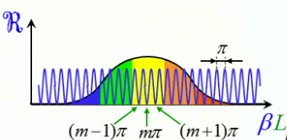
\includegraphics[scale=0.7]{ch4/image25.png}
	\captionof{figure}{ }
	\end{wrapfigure}
Pour un film centimétrique : $\Delta(\beta L) = 8\pi*10^3\cos\theta$. Cette extension est largement 
plus grande que $\pi$, il faut représenter un nombre d'ordre très élevé pour que la superposition 
donne quelque chose de visible. Le spectre visible englobe un très grand nombre de période de la 
fonction d'Airy en réflexion. C'était ce que l'on avait précédemment obtenu : le filme mince 
sélectionnait les longueurs d'onde extrêmement rapprochée : celles qui reste sont représentatives 
du spectre visible et il n'y a pas de phénomène d'irisation détectable à l’œil nu.


\newpage
\section{Le spectroscope de Fabry-Perot}
	\begin{wrapfigure}[13]{r}{5.5cm}
	\vspace{-8mm}
	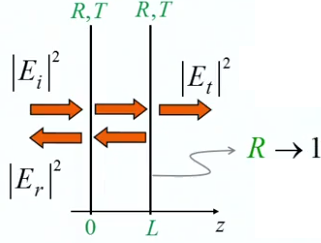
\includegraphics[scale=0.5]{ch4/image26.png}
	\captionof{figure}{ }
	\end{wrapfigure}
L'interféromètre de Fabry-Perot a été développé pour sa capacité à faire de l'analyse spectrale. 
Nous allons ici nous y intéresser, mais sous sa version moderne à travers de la transmission d'Airy. 
Le spectroscope va fonctionner à incidence normale, on va annuler l'angle $\theta$ apparaissant dans 
$\beta$
\begin{equation}
\beta = k\cos\theta \quad\rightarrow\quad \beta = k
\end{equation}
La fonction d'Airy devient
\begin{equation}
\mathcal{F} = \dfrac{1}{1+F\sin^2(kL)}
\end{equation}
Il ne faut donc plus se préoccuper de l'angle $\theta$, grande simplification. Autre précaution, 
nous considérons des miroirs de grande qualité et surtout de très grande réflectivité : $
R\rightarrow 1$, ce qui est faisable avec les techniques modernes. Ceci implique que la 
transmission tend vers zéro, $T\rightarrow0$.\\

La transmission de l'onde incidente est réduite à un très faible fraction, mais grâce aux aller-retour
nombreux dans la cavité, une onde d'intensité importante tel que l'intensité à la sortie vaudra 
celle à l'incidence ($\mathcal{T}=1$) et ce malgré une transmission ridiculement faible\footnote{On 
se rappelle que l'on a bien une transmission unitaire à la résonance et ce de façon indépendante de la 
réflexibilité (le sinus étant nul, le $R$ caché dans la finesse ne joue aucun rôle).}. \\

Après avoir lu la note en bas de page (héhé), intéressons-nous à la finesse
\begin{equation}
F = \frac{4R}{(1-R)^2}=\dfrac{4(1-T)}{T^2} \approx \frac{4}{T^2}
\end{equation}
Plus la transmission est petite, plus la finesse sera grande. Ceci sont les conditions d'utilisation 
pour faire du FB un spectroscope.\\

	\begin{wrapfigure}[8]{l}{5cm}
	\vspace{-8mm}
	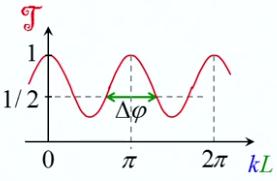
\includegraphics[scale=0.5]{ch4/image27.png}
	\captionof{figure}{ }
	\end{wrapfigure}
Par exemple, considérons $R=99\%\rightarrow T=0.01\rightarrow F\approx 4*10^4$. Ceci peut paraître 
énorme, mais il est possible aujourd'hui de faire encore mieux que ça. Un tel facteur va sensiblement 
modifier l'allure de la fonction d'Airy. Étudions l'allure des pics de résonance dans le cas d'une 
telle finesse. Définissions $\Delta\phi$ comme la largeur des résonances (celles-ci étant toutes 
identiques) à mi-hauteur. Il est possible de trouver simplement l'abscisse $\frac{\Delta \phi}{2}$ 
par simple lecture graphique. Comme celle-ci correspond à une hauteur 1/2, il va être possible de 
calculer $\Delta\phi$. Exprimé mathématique, nous obtenons
\begin{equation}
\mathcal{T} = \dfrac{1}{1+F\sin^2\left(\frac{\Delta\phi}{2}\right)}= \frac{1}{2}
\end{equation}
Pour obtenir le même dénominateur, il faut nécessairement que 
\begin{equation}
F\sin^2\left(\frac{\Delta\phi}{2}\right)=1\quad\Leftrightarrow\quad \sin^2\left(\frac{\Delta\phi}{2}\right)
=\dfrac{1}{F}
\end{equation}
Le sinus carré est forcément très petit dans la limite des finesses élevées : l'argument doit forcément 
être très petit également. En utilisant l'approximation du premier ordre (\danger\ attention au carré) :
\begin{equation}
\left(\frac{\Delta\phi}{2}\right) = \frac{1}{F}\quad\Leftrightarrow\quad \Delta\phi^2 = \frac{4}{F}
\end{equation}

	\begin{wrapfigure}[8]{r}{5cm}
	\vspace{-8mm}
	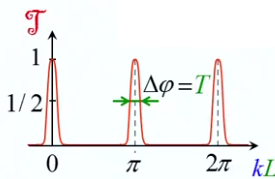
\includegraphics[scale=0.5]{ch4/image28.png}
	\captionof{figure}{ }
	\end{wrapfigure}
En utilisant l'approximation de la finesse faite ci-dessus
\begin{equation}
\Delta\phi^2 = T^2\quad\Leftrightarrow\quad \Delta\phi = T
\end{equation}
Ceci montre que les résonances exploitées en spectroscopies seront extrêmement larges. Les pics de 
la fonction d'Airy sont très fin, étroits, car la finesse est grande.\\

L'idée du spectroscope est de faire varier la longueur de la cavité du FP, $L$ (en plaçant le miroir 
sur une monture piezoélectrique). Nous allons donc maintenant nous intéressé à la variable $L$. Exprimons 
le graphe de la fonction d'Airy en fonction de la longueur $L$. Avec la condition de résonance 
\begin{equation}
kL = m\pi\quad\Rightarrow\quad L=\frac{m\pi}{k} = \frac{m\pi}{2\pi}\lambda=\frac{m\lambda}{2}
\end{equation}

	\begin{wrapfigure}[9]{l}{7cm}
	\vspace{-8mm}
	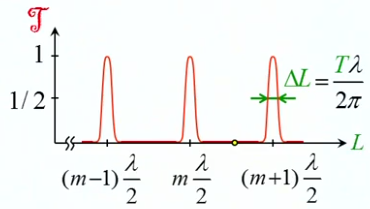
\includegraphics[scale=0.5]{ch4/image29.png}
	\captionof{figure}{ }
	\end{wrapfigure}
$L$ est un nombre demi-entier de longueur d'onde pour avoir une résonance, soit les pics de l'illustration 
ci-dessus. Pour faire la représentation, il suffit de changer la variable $kL$ en $L$ pour voir 
apparaître un pic tous les multiples de demi longueur d'onde. On pourrait s'intéresser à la largeur de la 
résonance en fonction de $L$. Il suffit pour ça de voir que
\begin{equation}
\Delta\phi = k\Delta L = \frac{2\pi}{\lambda}\Delta L = T\quad\Leftrightarrow\quad \Delta L = \frac{T\lambda}{
2\pi}
\end{equation}


Ceci étant dit, nous allons pouvoir nous intéresser à la physique lorsque $L$ se voit modifié. Le point 
de fonctionnement (au jaune ci-dessus) va effectuer des allers-retours sur un pics de résonance lorsque 
$L$ est modifié : l'intensité transmise s’éteint et s'allume de l'autre côté du miroir.\\

	\begin{wrapfigure}[9]{r}{3.5cm}
	\vspace{-8mm}
	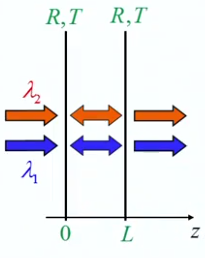
\includegraphics[scale=0.5]{ch4/image30.png}
	\captionof{figure}{ }
	\end{wrapfigure}
Nous pouvons maintenant aborder la spectroscopie du FP. Considérons une situation simple : deux longueurs 
d'onde présentes dans un faisceau lumineux, où $\lambda_2>\lambda_1$. Dans le graphique de la fonction 
d'Airy, il fait alors considérer deux pics de résonance. La largeur de la résonance s'exprime toujours 
comme $\Delta L = \frac{T\overline{\lambda}}{2\pi}$ où $\overline{\lambda}$ est la longueur d'onde moyenne.

On peut à nouveau considérer une modification de $L$ : le balayage (le petit point jaune) va maintenant 
passer par les deux pics, qui n'apparaissent pas ensemble mais en alternance. Comment réussir à exploiter 
quelque chose de ceci ? Ci-dessous, le dispositif mis en œuvre
\newpage
\begin{center}
	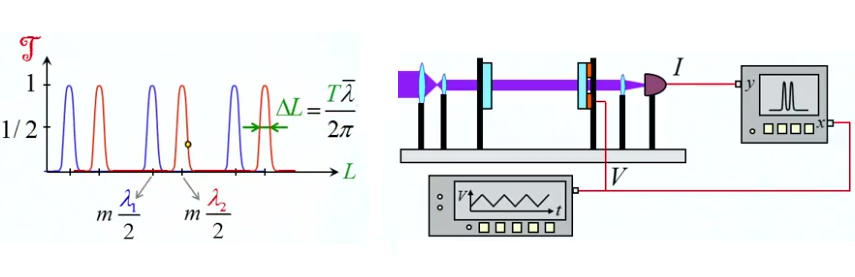
\includegraphics[scale=0.5]{ch4/image31.png}
	\captionof{figure}{ }
\end{center}
On y voit le FP où le miroir de droite est sur sa monture piezométrique qui est elle-même reliée à 
un générateur de tension (permettant de modifier $L$ à l'échelle du micron) fournissant un signal 
triangulaire. Avec un capteur d'intensité, on récupère une tension du aux flash successifs émis en 
alternance par le FP. Cette tension est mise en mode $y$ d'un oscilloscope alors que celle servant 
à la monture piezométrique est mise en mode $x$ (donne une droite horizontale) de façon à exploiter 
le mode $xy$ pour se débarrasser de l'axe temporel.\\

	\begin{wrapfigure}[9]{r}{7.5cm}
	\vspace{-8mm}
	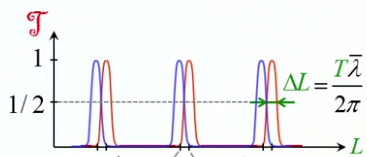
\includegraphics[scale=0.6]{ch4/image32.png}
	\captionof{figure}{ }
	\end{wrapfigure}
On relève ainsi le contenu spectral de la lumière incidente sur le FP. On a réussi à reconstituer 
l'allure de $\mathcal{T}$. Ceci est fait pour deux longueurs d'onde, c'est bien entendu généralisable 
à un grand nombre de longueurs d'onde. Étudions maintenant la résolution de ce spectre. Les 
spectroscopiste ont défini une limite : les deux résonances se rapprochent au plus tel qu'elles se 
croisent à mi-hauteur, il s'agit de la limite de résolution. A cet endroit la on arrive encore à 
distinguer les deux longueurs d'onde mais après l'incertitude devient trop importante. Cette limite 
de résolution s'exprime
\begin{equation}
\left|m\dfrac{\lambda_1}{2}-m\dfrac{\lambda_2}{2}\right|_{\min} \equiv \dfrac{T\overline{\lambda}}{2\pi}
\end{equation}
Soit la largeur à mi-hauteur en première approximation. En peut en trier
\begin{equation}
\dfrac{m}{2}\Delta\lambda_{\min} \equiv\dfrac{T\overline{\lambda}}{2\pi}
\end{equation}
où $\Delta\lambda_{\min}$ est l'écart de longueur d'onde minimale que l'on peut résoudre avec le 
spectroscope. La résolution d'une spectromètre s'exprime alors
\begin{equation}
\mathcal{R} \equiv\dfrac{\Delta\lambda_{\min}}{\overline{\lambda}} = \dfrac{T}{m\pi}
\end{equation}
Ceci est un peu abstrait à cause de la présence du $m$ : comment connaître l'ordre de la résonance ? 
Si on étudie les précédents pics, nous savons que $\DS\frac{m\overline{\lambda}}{2}\approx L$. Dès 
lors $\DS m\approx \frac{2L}{\overline{\lambda}}$ et la résolution devient
\begin{equation}
\mathcal{R} \equiv\dfrac{\Delta\lambda_{\min}}{\overline{\lambda}} =\dfrac{T}{2\pi}\dfrac{\overline{\lambda}}{L}
\end{equation}\ \\

\newpage
	\begin{wrapfigure}[6]{r}{2.5cm}
	\vspace{-3mm}
	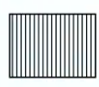
\includegraphics[scale=0.6]{ch4/image33.png}
	\captionof{figure}{ }
	\end{wrapfigure}
Illustrions avec le même exemple que précédemment ($L=\ 10cm, \overline{\lambda}=0.5\ \mu m, T=0.01, 
F=4*10^4$). On obtient pour ces valeurs $\mathcal{R} = 0.75*10^{-8}$. Cette résolution est classique 
pour un FP. Comparons cette résolution avec celle des réseaux de diffraction (une plaque gravée avec 
des traits séparées d'un certains pas). Un tel réseau possède une résolution $\mathcal{R}=\frac{1}{N}$ 
où $N$ est le nombre de traits du réseaux. Si l'on considère $p\approx 1\ \mu m.$ Pour avoir la même 
résolution que notre FB, il faut que $N\approx 10^8$. Ceci donne un réseau qui à une longueur de 
100m ($Np=10^2$ m) ce qui ne se fait pas en pratique. Le FP est nettement supérieur en terme de 
résolution que le réseau de diffraction.\\

	\begin{wrapfigure}[11]{l}{7.5cm}
	\vspace{-5mm}
	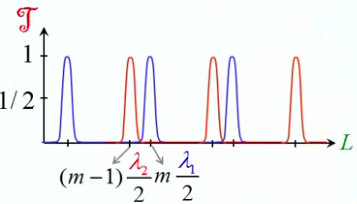
\includegraphics[scale=0.6]{ch4/image34.png}
	\captionof{figure}{ }
	\end{wrapfigure}
Pourquoi continuer d'utiliser ce dernier? Le FP est excellent 
pour étudier la finesse des pics de résonance mais il n'est adapté qu'aux détails spectraux extrêmement 
fins. Le spectre est en réalité périodique (d'une demi longueur d'onde) et le FB n'en observe qu'un seul. 
Essayons d'observer deux longueurs d'ondes qui ne sont ni trop rapprochées, ni trop éloignées. Volontairement, 
le pic de la résonance correspondant à la longueur d'onde $\lambda_2$ est représenté par l'ordre $(m-1)$.
Si $\lambda_1$ et $\lambda_2$ s'éloignent trop l'un de l'autre, le pic de l'ordre $(m-1)$ va se rapprocher 
du pic de l'ordre $m$. Or l'ordre n'est pas connu, quand on relèvera l'ensemble de pics à l'oscilloscope 
on pourrait mal l'interpréter physiquement n'ayant pas accès à l'ordre de la résonance.\\

Un FB doit toujours être utilisé tel que les ordres soit bien distincts l'un de l'autre. Il faut donc
\begin{equation}
(m-1)\frac{\lambda_2}{2}<m\frac{\lambda_1}{2}\quad\Leftrightarrow\quad m(\lambda_2-\lambda_1)<\lambda_2
\end{equation}
Traduisons cette relation pour voir ce qu'elle devient en terme de longueur accessibles par le FP. 
Comme d'habitude, nous n'avons pas accès à $m$. Il faut alors  utiliser $m\approx \frac{2L}{\overline{
\lambda}}$. En remplaçant $\lambda_2$ par $\overline{\lambda}$ (on étudie la largeur de spectre qui, 
étant extrêmement fine, autorise ce changement)
\begin{equation}
\Delta \lambda <\dfrac{\overline{\lambda}^2}{2L}
\end{equation}
où $\Delta \lambda$ est la largeur spectrale accessible au FP. Ceci est très limitant. Un exemple 
valant mieux qu'un long discours
\begin{equation}
\left\{\begin{array}{ll}
\overline{\lambda} &= 0.5\ \mu m\\
L &= 10\ cm
\end{array}\right.\quad\Rightarrow\quad \Delta \lambda < 10^{-6}\ \mu m 
\end{equation}
Le FB est bien pour étudier des détails extrêmement fin mais le réseau de diffraction reste 
intéressant pour l'étude de spectres larges. 





























